Task B2 was to implement process handling in our operating system. Lets look a bit closer on the concept of processes before discussing the implementation.
\subsection{The process concept}
A process is a in an instance of a program (an executable) that runs in an operating system environment, 
and returns to this operating system upon completion. Hence, the operating system is the one responsible for 
creating new processes and terminating them. An analogy to this is the a java object, being an instance of a java class.\\
The process is therefore nothing more than a container for resources reserved to the process by the operating system. \\

\subsection{The thread concept}
A thread is the part of the process container responsible for executing the program. Usually processes can have a number of threads as illustrated in figure \ref{fig:thread_models}.(a). \\

So, the operating system need to keep track of the running processes and take care of creating and terminating the processes. 
For this, we have added two system calls; create and terminate.

\begin{figure}
\centering
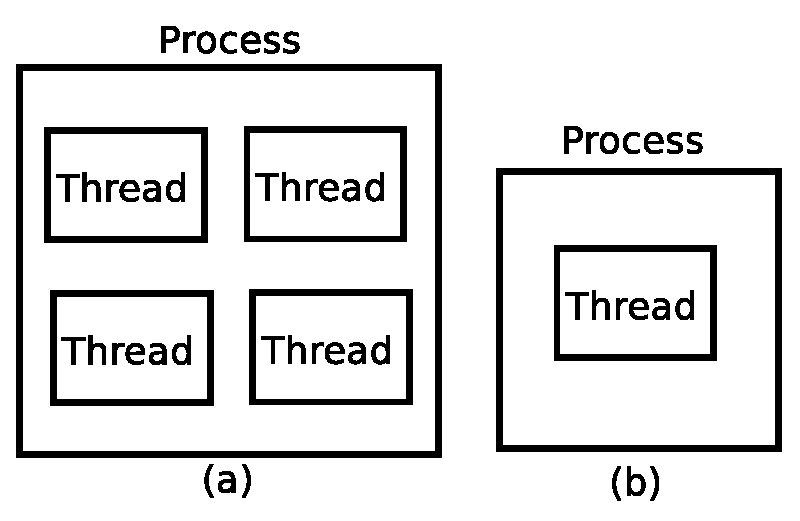
\epsfig{file=fig/Thread_Models.eps, height=1in}
\caption{Typical thread models}
\label{fig:thread_models}
\end{figure}

\subsubsection*{The create system call}
To to keep track of the running processes we maintain process table that contains structures holding information about an individual process. \\
Processes are executed invoking this system call by executing a piece of assembler code that calls a named procedure called ``main'' and then calls terminate when main is done executing. In this system call we create one thread, and only one for each process, so our thread model actually looks like figure \ref{fig:thread_models}.(b)

\subsubsection*{The terminate system call}
When a program finishes the terminate system call is invoked. This call does a clean-up by, of course, cleaning up references to the process 
and the threads of the process. Then finally do a context switch. By doing so, we run the next thread in the ready queue.

\subsection{Reflections}

\subsubsection*{How is the system booted?}
Our virtual pc starts a BIOS that searches for a bootloader (in our case Grub), that then loads the kernel image to memory from a harddisk - or in our case a disk image. The virtual pc is an AMD64 architecture. The PC starts up in real mode, goes to protected mode and finally to long mode. Real mode is the legacy real address mode used by the original Intel 8086 CPU's. Protected mode is the legacy protected virtual address mode that supports virtual memory and paging. Long mode is standard x86-64 mode used when

\subsubsection*{How are processes created from executable files?}
The kernel loads all executable programs along with it, storing a pointer to the first instruction for each process. The function prepare\_process does a lot of sanity checks on the image assuring that it is in fact meant for execution. So every process is with the kernel when it is started and to add additional would require a recompilation and reboot.

\subsubsection*{How does a daemon (process) differ from processes studied in this task?}
Our processes runs ``interactively'' and daemons traditionally run in the background. Otherwise they share the fact that they are started at bootup by the operating system. In LInux processes become daemons by forking a child process and make the parent process exit, this causes init to adopt the child process.

\subsection{Test}
This task needs to have implemented the system calls ``createprocess'' and ``terminate'' so that the two executables are able to create process as stored in the executable\_table. After the executables have reached the end of their code they will make the system call to terminate. This desired result was achieved as defined in task definition, and the test was a success.